% Options for packages loaded elsewhere
\PassOptionsToPackage{unicode}{hyperref}
\PassOptionsToPackage{hyphens}{url}
%
\documentclass[
]{article}
\usepackage{lmodern}
\usepackage{amssymb,amsmath}
\usepackage{ifxetex,ifluatex}
\ifnum 0\ifxetex 1\fi\ifluatex 1\fi=0 % if pdftex
  \usepackage[T1]{fontenc}
  \usepackage[utf8]{inputenc}
  \usepackage{textcomp} % provide euro and other symbols
\else % if luatex or xetex
  \usepackage{unicode-math}
  \defaultfontfeatures{Scale=MatchLowercase}
  \defaultfontfeatures[\rmfamily]{Ligatures=TeX,Scale=1}
\fi
% Use upquote if available, for straight quotes in verbatim environments
\IfFileExists{upquote.sty}{\usepackage{upquote}}{}
\IfFileExists{microtype.sty}{% use microtype if available
  \usepackage[]{microtype}
  \UseMicrotypeSet[protrusion]{basicmath} % disable protrusion for tt fonts
}{}
\makeatletter
\@ifundefined{KOMAClassName}{% if non-KOMA class
  \IfFileExists{parskip.sty}{%
    \usepackage{parskip}
  }{% else
    \setlength{\parindent}{0pt}
    \setlength{\parskip}{6pt plus 2pt minus 1pt}}
}{% if KOMA class
  \KOMAoptions{parskip=half}}
\makeatother
\usepackage{xcolor}
\IfFileExists{xurl.sty}{\usepackage{xurl}}{} % add URL line breaks if available
\IfFileExists{bookmark.sty}{\usepackage{bookmark}}{\usepackage{hyperref}}
\hypersetup{
  pdftitle={Inference for Numerical Data},
  pdfauthor={Zachary Palmore},
  hidelinks,
  pdfcreator={LaTeX via pandoc}}
\urlstyle{same} % disable monospaced font for URLs
\usepackage[margin=1in]{geometry}
\usepackage{color}
\usepackage{fancyvrb}
\newcommand{\VerbBar}{|}
\newcommand{\VERB}{\Verb[commandchars=\\\{\}]}
\DefineVerbatimEnvironment{Highlighting}{Verbatim}{commandchars=\\\{\}}
% Add ',fontsize=\small' for more characters per line
\usepackage{framed}
\definecolor{shadecolor}{RGB}{248,248,248}
\newenvironment{Shaded}{\begin{snugshade}}{\end{snugshade}}
\newcommand{\AlertTok}[1]{\textcolor[rgb]{0.94,0.16,0.16}{#1}}
\newcommand{\AnnotationTok}[1]{\textcolor[rgb]{0.56,0.35,0.01}{\textbf{\textit{#1}}}}
\newcommand{\AttributeTok}[1]{\textcolor[rgb]{0.77,0.63,0.00}{#1}}
\newcommand{\BaseNTok}[1]{\textcolor[rgb]{0.00,0.00,0.81}{#1}}
\newcommand{\BuiltInTok}[1]{#1}
\newcommand{\CharTok}[1]{\textcolor[rgb]{0.31,0.60,0.02}{#1}}
\newcommand{\CommentTok}[1]{\textcolor[rgb]{0.56,0.35,0.01}{\textit{#1}}}
\newcommand{\CommentVarTok}[1]{\textcolor[rgb]{0.56,0.35,0.01}{\textbf{\textit{#1}}}}
\newcommand{\ConstantTok}[1]{\textcolor[rgb]{0.00,0.00,0.00}{#1}}
\newcommand{\ControlFlowTok}[1]{\textcolor[rgb]{0.13,0.29,0.53}{\textbf{#1}}}
\newcommand{\DataTypeTok}[1]{\textcolor[rgb]{0.13,0.29,0.53}{#1}}
\newcommand{\DecValTok}[1]{\textcolor[rgb]{0.00,0.00,0.81}{#1}}
\newcommand{\DocumentationTok}[1]{\textcolor[rgb]{0.56,0.35,0.01}{\textbf{\textit{#1}}}}
\newcommand{\ErrorTok}[1]{\textcolor[rgb]{0.64,0.00,0.00}{\textbf{#1}}}
\newcommand{\ExtensionTok}[1]{#1}
\newcommand{\FloatTok}[1]{\textcolor[rgb]{0.00,0.00,0.81}{#1}}
\newcommand{\FunctionTok}[1]{\textcolor[rgb]{0.00,0.00,0.00}{#1}}
\newcommand{\ImportTok}[1]{#1}
\newcommand{\InformationTok}[1]{\textcolor[rgb]{0.56,0.35,0.01}{\textbf{\textit{#1}}}}
\newcommand{\KeywordTok}[1]{\textcolor[rgb]{0.13,0.29,0.53}{\textbf{#1}}}
\newcommand{\NormalTok}[1]{#1}
\newcommand{\OperatorTok}[1]{\textcolor[rgb]{0.81,0.36,0.00}{\textbf{#1}}}
\newcommand{\OtherTok}[1]{\textcolor[rgb]{0.56,0.35,0.01}{#1}}
\newcommand{\PreprocessorTok}[1]{\textcolor[rgb]{0.56,0.35,0.01}{\textit{#1}}}
\newcommand{\RegionMarkerTok}[1]{#1}
\newcommand{\SpecialCharTok}[1]{\textcolor[rgb]{0.00,0.00,0.00}{#1}}
\newcommand{\SpecialStringTok}[1]{\textcolor[rgb]{0.31,0.60,0.02}{#1}}
\newcommand{\StringTok}[1]{\textcolor[rgb]{0.31,0.60,0.02}{#1}}
\newcommand{\VariableTok}[1]{\textcolor[rgb]{0.00,0.00,0.00}{#1}}
\newcommand{\VerbatimStringTok}[1]{\textcolor[rgb]{0.31,0.60,0.02}{#1}}
\newcommand{\WarningTok}[1]{\textcolor[rgb]{0.56,0.35,0.01}{\textbf{\textit{#1}}}}
\usepackage{graphicx,grffile}
\makeatletter
\def\maxwidth{\ifdim\Gin@nat@width>\linewidth\linewidth\else\Gin@nat@width\fi}
\def\maxheight{\ifdim\Gin@nat@height>\textheight\textheight\else\Gin@nat@height\fi}
\makeatother
% Scale images if necessary, so that they will not overflow the page
% margins by default, and it is still possible to overwrite the defaults
% using explicit options in \includegraphics[width, height, ...]{}
\setkeys{Gin}{width=\maxwidth,height=\maxheight,keepaspectratio}
% Set default figure placement to htbp
\makeatletter
\def\fps@figure{htbp}
\makeatother
\setlength{\emergencystretch}{3em} % prevent overfull lines
\providecommand{\tightlist}{%
  \setlength{\itemsep}{0pt}\setlength{\parskip}{0pt}}
\setcounter{secnumdepth}{-\maxdimen} % remove section numbering

\title{Inference for Numerical Data}
\author{Zachary Palmore}
\date{2020-10-18}

\begin{document}
\maketitle

\begin{Shaded}
\begin{Highlighting}[]
\KeywordTok{library}\NormalTok{(tidyverse)}
\KeywordTok{library}\NormalTok{(openintro)}
\KeywordTok{library}\NormalTok{(infer)}
\KeywordTok{library}\NormalTok{(statsr)}
\KeywordTok{library}\NormalTok{(psych)}
\end{Highlighting}
\end{Shaded}

\hypertarget{pre-exercise}{%
\subsubsection{Pre-exercise}\label{pre-exercise}}

Loading the data for this lab.

Looking at the meaning of variables.

\begin{Shaded}
\begin{Highlighting}[]
\NormalTok{?yrbss}
\end{Highlighting}
\end{Shaded}

\hypertarget{exercise-1}{%
\subsubsection{Exercise 1}\label{exercise-1}}

What are the cases in this data set? How many cases are there in our
sample?

\begin{Shaded}
\begin{Highlighting}[]
\KeywordTok{glimpse}\NormalTok{(yrbss)}
\end{Highlighting}
\end{Shaded}

\begin{verbatim}
## Rows: 13,583
## Columns: 13
## $ age                      <int> 14, 14, 15, 15, 15, 15, 15, 14, 15, 15, 15...
## $ gender                   <chr> "female", "female", "female", "female", "f...
## $ grade                    <chr> "9", "9", "9", "9", "9", "9", "9", "9", "9...
## $ hispanic                 <chr> "not", "not", "hispanic", "not", "not", "n...
## $ race                     <chr> "Black or African American", "Black or Afr...
## $ height                   <dbl> NA, NA, 1.73, 1.60, 1.50, 1.57, 1.65, 1.88...
## $ weight                   <dbl> NA, NA, 84.37, 55.79, 46.72, 67.13, 131.54...
## $ helmet_12m               <chr> "never", "never", "never", "never", "did n...
## $ text_while_driving_30d   <chr> "0", NA, "30", "0", "did not drive", "did ...
## $ physically_active_7d     <int> 4, 2, 7, 0, 2, 1, 4, 4, 5, 0, 0, 0, 4, 7, ...
## $ hours_tv_per_school_day  <chr> "5+", "5+", "5+", "2", "3", "5+", "5+", "5...
## $ strength_training_7d     <int> 0, 0, 0, 0, 1, 0, 2, 0, 3, 0, 3, 0, 0, 7, ...
## $ school_night_hours_sleep <chr> "8", "6", "<5", "6", "9", "8", "9", "6", "...
\end{verbatim}

There at 13,583 rows which is also the number of cases in this sample.
The 13 cases in this data set were listed as:

\begin{verbatim}
* age
* gender
* grade
* hispanic
* race
* height
* weight
* helmet_12m
* text_while_driving_30d
* physically_active_7d 
* hours_tv_per_school_day
* strength_training_7d
* school_night_hours_sleep 
\end{verbatim}

\hypertarget{exercise-2}{%
\subsubsection{Exercise 2}\label{exercise-2}}

How many observations are we missing weights from?

Altogether, there are 9,476 missing values.

\begin{Shaded}
\begin{Highlighting}[]
\KeywordTok{sum}\NormalTok{(}\KeywordTok{is.na}\NormalTok{(yrbss))}
\end{Highlighting}
\end{Shaded}

\begin{verbatim}
## [1] 9476
\end{verbatim}

Under the observations of \emph{weights} we have 1004 missing values.

\begin{Shaded}
\begin{Highlighting}[]
\KeywordTok{sum}\NormalTok{(}\KeywordTok{is.na}\NormalTok{(yrbss}\OperatorTok{$}\NormalTok{weight))}
\end{Highlighting}
\end{Shaded}

\begin{verbatim}
## [1] 1004
\end{verbatim}

We could also use the summary function which confirms these missing
values as the total number of NA in each column and provides some basic
statistics. Here, we selected the weight column from the cases.

\begin{Shaded}
\begin{Highlighting}[]
\KeywordTok{summary}\NormalTok{(yrbss[,}\DecValTok{7}\NormalTok{])}
\end{Highlighting}
\end{Shaded}

\begin{verbatim}
##      weight      
##  Min.   : 29.94  
##  1st Qu.: 56.25  
##  Median : 64.41  
##  Mean   : 67.91  
##  3rd Qu.: 76.20  
##  Max.   :180.99  
##  NA's   :1004
\end{verbatim}

\hypertarget{exercise-3}{%
\subsubsection{Exercise 3}\label{exercise-3}}

Make a side-by-side boxplot of physical\_3plus and weight. Is there a
relationship between these two variables? What did you expect and why?

Creating the variable \emph{physical\_3plus} and filling in the case
values with ``yes'' if the individual was physically active for at least
3 days in the week or ``no'' if they were not.

\begin{Shaded}
\begin{Highlighting}[]
\NormalTok{yrbss <-}\StringTok{ }\NormalTok{yrbss }\OperatorTok\StringTok{ }
\StringTok{  }\KeywordTok{mutate}\NormalTok{(}\DataTypeTok{physical_3plus =} \KeywordTok{ifelse}\NormalTok{(yrbss}\OperatorTok{$}\NormalTok{physically_active_7d }\OperatorTok{>}\StringTok{ }\DecValTok{2}\NormalTok{, }\StringTok{"yes"}\NormalTok{, }\StringTok{"no"}\NormalTok{)) }
\end{Highlighting}
\end{Shaded}

A side-by-side boxplot will be made but keep in mind the missing
variables listed as ``NA'' in the data frame are also plotted.

\begin{Shaded}
\begin{Highlighting}[]
\KeywordTok{sum}\NormalTok{(}\KeywordTok{is.na}\NormalTok{(yrbss}\OperatorTok{$}\NormalTok{physical_3plus))}
\end{Highlighting}
\end{Shaded}

\begin{verbatim}
## [1] 273
\end{verbatim}

There are 273 of them which is a small proportion of the number of
observations overall.

\begin{Shaded}
\begin{Highlighting}[]
\KeywordTok{ggplot}\NormalTok{(yrbss, }\KeywordTok{aes}\NormalTok{(}\DataTypeTok{x=}\NormalTok{weight, }\DataTypeTok{y=}\NormalTok{physical_3plus)) }\OperatorTok{+}\StringTok{ }\KeywordTok{geom_boxplot}\NormalTok{() }\OperatorTok{+}\StringTok{ }\KeywordTok{theme_bw}\NormalTok{()}
\end{Highlighting}
\end{Shaded}

\begin{verbatim}
## Warning: Removed 1004 rows containing non-finite values (stat_boxplot).
\end{verbatim}

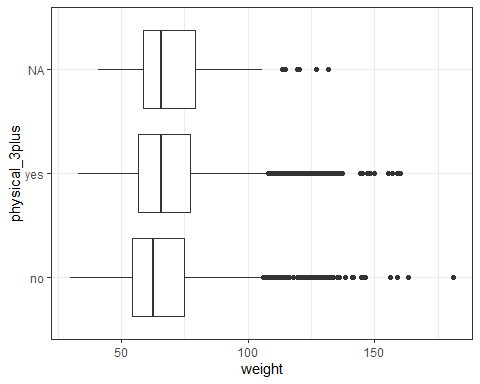
\includegraphics{Lab-7---Inference-for-Numerical-Data_files/figure-latex/unnamed-chunk-9-1.pdf}

We could remove these from the data frame entirely by adding to a
parameter to the chink where the \emph{physical\_3plus} column was
created then plot again.

\begin{Shaded}
\begin{Highlighting}[]
\NormalTok{yrbss2 <-}\StringTok{ }\NormalTok{yrbss }\OperatorTok\StringTok{ }
\StringTok{  }\KeywordTok{mutate}\NormalTok{(}\DataTypeTok{physical_3plus =} \KeywordTok{ifelse}\NormalTok{(yrbss}\OperatorTok{$}\NormalTok{physically_active_7d }\OperatorTok{>}\StringTok{ }\DecValTok{2}\NormalTok{, }\StringTok{"yes"}\NormalTok{, }\StringTok{"no"}\NormalTok{)) }\OperatorTok
\StringTok{  }\KeywordTok{na.exclude}\NormalTok{()}
\KeywordTok{ggplot}\NormalTok{(yrbss2, }\KeywordTok{aes}\NormalTok{(}\DataTypeTok{x=}\NormalTok{weight, }\DataTypeTok{y=}\NormalTok{physical_3plus)) }\OperatorTok{+}\StringTok{ }\KeywordTok{geom_boxplot}\NormalTok{() }\OperatorTok{+}\StringTok{ }\KeywordTok{theme_bw}\NormalTok{()}
\end{Highlighting}
\end{Shaded}

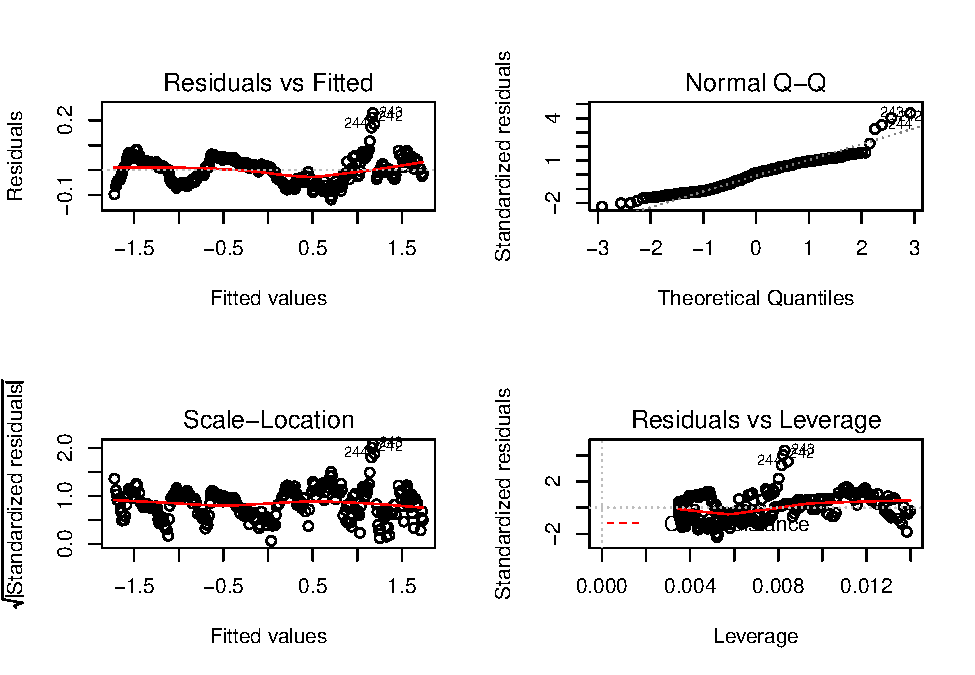
\includegraphics{Lab-7---Inference-for-Numerical-Data_files/figure-latex/unnamed-chunk-10-1.pdf}

The relationship between a student's weight and if they are physically
active at least 3 times per week seems to show that those who are not
physically active at least 3 times per week weigh less than those who
are physically active at least 3 times per week. This is interesting as
I would have expected those who were physically active at least 3 times
per week to weigh less than those who were not physically active at
least 3 times per week. My assumption comes from the idea that being
physically active burns calories and fat, which over time, reduces a
person's weight. Although, these results are contrary to that
assumption.

We can check the statistics by comparing numeric values as well.

\begin{Shaded}
\begin{Highlighting}[]
\NormalTok{yrbss }\OperatorTok
\StringTok{  }\KeywordTok{group_by}\NormalTok{(physical_3plus) }\OperatorTok
\StringTok{  }\KeywordTok{summarise}\NormalTok{(}\DataTypeTok{mean_weight =} \KeywordTok{mean}\NormalTok{(weight, }\DataTypeTok{na.rm =} \OtherTok{TRUE}\NormalTok{))}
\end{Highlighting}
\end{Shaded}

\begin{verbatim}
## `summarise()` ungrouping output (override with `.groups` argument)
\end{verbatim}

\begin{verbatim}
## # A tibble: 3 x 2
##   physical_3plus mean_weight
##   <chr>                <dbl>
## 1 no                    66.7
## 2 yes                   68.4
## 3 <NA>                  69.9
\end{verbatim}

With this, the relationship continues. Those who are physically active
at least 3 days per week have a higher mean weight at 68.45 kg than
those who are not physically active at least 3 times per week at 66.67
kg.

\hypertarget{exercise-4}{%
\subsubsection{Exercise 4}\label{exercise-4}}

Are all conditions necessary for inference satisfied? Comment on each.
You can compute the group sizes with the summarize command above by
defining a new variable with the definition n().

There are two conditions, independence and normality. Based on the
information from the CDC, the data is a representative sample of many
students across national, state, tribal, and local school systems and is
independent. To determine normality we can look at the sample size and
distribution of the boxplots. With a sample size well over 1000 (the
threshold is 30) and no particularly extreme outliers, we can assume the
normality condition is satisfied. The sample size of the weights is
calculated by physical activity below.

\begin{Shaded}
\begin{Highlighting}[]
\NormalTok{yrbss }\OperatorTok\StringTok{ }
\StringTok{  }\KeywordTok{group_by}\NormalTok{(physical_3plus) }\OperatorTok\StringTok{ }
\StringTok{  }\KeywordTok{summarise}\NormalTok{(}\DataTypeTok{freq =} \KeywordTok{table}\NormalTok{(weight)) }\OperatorTok
\StringTok{  }\KeywordTok{summarise}\NormalTok{(}\DataTypeTok{n =} \KeywordTok{sum}\NormalTok{(freq))}
\end{Highlighting}
\end{Shaded}

\begin{verbatim}
## `summarise()` regrouping output by 'physical_3plus' (override with `.groups` argument)
\end{verbatim}

\begin{verbatim}
## `summarise()` ungrouping output (override with `.groups` argument)
\end{verbatim}

\begin{verbatim}
## # A tibble: 3 x 2
##   physical_3plus     n
##   <chr>          <int>
## 1 no              4022
## 2 yes             8342
## 3 <NA>             215
\end{verbatim}

\hypertarget{exercise-5}{%
\subsubsection{Exercise 5}\label{exercise-5}}

Write the hypotheses for testing if the average weights are different
for those who exercise at least times a week and those who don't.

Null hypothesis: Students who are physically active 3 or more days per
week have the same average weight as those who are not physically active
3 or more days per week.

Alternative hypothesis: Students who are physically active 3 or more
days per week have a different average weight when compared to those who
are not physically active 3 or more days per week.

\hypertarget{exercise-6}{%
\subsubsection{Exercise 6}\label{exercise-6}}

How many of these null permutations have a difference of at least
obs\_stat?

From lab we begin by initializing the test,

\begin{Shaded}
\begin{Highlighting}[]
\NormalTok{obs_diff <-}\StringTok{ }\NormalTok{yrbss }\OperatorTok
\StringTok{  }\KeywordTok{specify}\NormalTok{(weight }\OperatorTok{~}\StringTok{ }\NormalTok{physical_3plus) }\OperatorTok
\StringTok{  }\KeywordTok{calculate}\NormalTok{(}\DataTypeTok{stat =} \StringTok{"diff in means"}\NormalTok{, }\DataTypeTok{order =} \KeywordTok{c}\NormalTok{(}\StringTok{"yes"}\NormalTok{, }\StringTok{"no"}\NormalTok{))}
\end{Highlighting}
\end{Shaded}

\begin{verbatim}
## Warning: Removed 1219 rows containing missing values.
\end{verbatim}

simulating test on null and then visualizing the results.

\begin{Shaded}
\begin{Highlighting}[]
\KeywordTok{set.seed}\NormalTok{(}\DecValTok{10142020}\NormalTok{)}
\NormalTok{null_dist <-}\StringTok{ }\NormalTok{yrbss }\OperatorTok
\StringTok{  }\KeywordTok{specify}\NormalTok{(weight }\OperatorTok{~}\StringTok{ }\NormalTok{physical_3plus) }\OperatorTok
\StringTok{  }\KeywordTok{hypothesize}\NormalTok{(}\DataTypeTok{null =} \StringTok{"independence"}\NormalTok{) }\OperatorTok
\StringTok{  }\KeywordTok{generate}\NormalTok{(}\DataTypeTok{reps =} \DecValTok{1000}\NormalTok{, }\DataTypeTok{type =} \StringTok{"permute"}\NormalTok{) }\OperatorTok
\StringTok{  }\KeywordTok{calculate}\NormalTok{(}\DataTypeTok{stat =} \StringTok{"diff in means"}\NormalTok{, }\DataTypeTok{order =} \KeywordTok{c}\NormalTok{(}\StringTok{"yes"}\NormalTok{, }\StringTok{"no"}\NormalTok{))}
\end{Highlighting}
\end{Shaded}

\begin{verbatim}
## Warning: Removed 1219 rows containing missing values.
\end{verbatim}

\begin{Shaded}
\begin{Highlighting}[]
\KeywordTok{visualize}\NormalTok{(null_dist) }\OperatorTok{+}\StringTok{ }
\StringTok{  }\KeywordTok{shade_p_value}\NormalTok{(}\DataTypeTok{obs_stat =}\NormalTok{ obs_diff, }\DataTypeTok{direction =} \StringTok{"two_sided"}\NormalTok{)}
\end{Highlighting}
\end{Shaded}

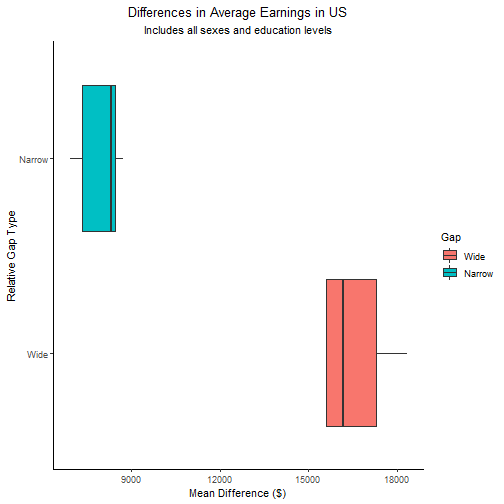
\includegraphics{Lab-7---Inference-for-Numerical-Data_files/figure-latex/unnamed-chunk-14-1.pdf}

Using the red line as a mark of the obs\_stat, it appears to far from
the data to have any values at or above it. To find the quantity of null
permutations that have a difference of at least obs\_stat we can filter
the stat values in the null\_dist data to show the total of those that
are greater than or equal to obs\_stat.

\begin{Shaded}
\begin{Highlighting}[]
\NormalTok{null_dist }\OperatorTok
\StringTok{  }\KeywordTok{filter}\NormalTok{(stat }\OperatorTok{>=}\StringTok{ }\NormalTok{obs_diff)}
\end{Highlighting}
\end{Shaded}

\begin{verbatim}
## # A tibble: 0 x 2
## # ... with 2 variables: replicate <int>, stat <dbl>
\end{verbatim}

We could also sum the number of stat values in null\_dist that are
greater. Both produce the same result.

\begin{Shaded}
\begin{Highlighting}[]
\KeywordTok{sum}\NormalTok{(null_dist}\OperatorTok{$}\NormalTok{stat }\OperatorTok{>=}\StringTok{ }\NormalTok{obs_diff}\OperatorTok{$}\NormalTok{stat)}
\end{Highlighting}
\end{Shaded}

\begin{verbatim}
## [1] 0
\end{verbatim}

To check the p-value we can use the get\_p\_value function.

\begin{Shaded}
\begin{Highlighting}[]
\NormalTok{null_dist }\OperatorTok
\StringTok{  }\KeywordTok{get_p_value}\NormalTok{(}\DataTypeTok{obs_stat =}\NormalTok{ obs_diff, }\DataTypeTok{direction =} \StringTok{"two_sided"}\NormalTok{)}
\end{Highlighting}
\end{Shaded}

\begin{verbatim}
## Warning: Please be cautious in reporting a p-value of 0. This result is an
## approximation based on the number of `reps` chosen in the `generate()` step. See
## `?get_p_value()` for more information.
\end{verbatim}

\begin{verbatim}
## # A tibble: 1 x 1
##   p_value
##     <dbl>
## 1       0
\end{verbatim}

The result is a very small number, approximately zero for practical
purposes.

\hypertarget{exercise-7}{%
\subsubsection{Exercise 7}\label{exercise-7}}

Construct and record a confidence interval for the difference between
the weights of those who exercise at least three times a week and those
who don't, and interpret this interval in context of the data.

\begin{Shaded}
\begin{Highlighting}[]
\KeywordTok{inference}\NormalTok{(}\DataTypeTok{data =}\NormalTok{ yrbss, }\DataTypeTok{y =}\NormalTok{ weight, }\DataTypeTok{x =}\NormalTok{ physical_3plus,}
          \DataTypeTok{statistic =} \StringTok{"mean"}\NormalTok{,}
          \DataTypeTok{type =} \StringTok{"ci"}\NormalTok{, }
          \DataTypeTok{null =} \OtherTok{NULL}\NormalTok{, }
          \DataTypeTok{alternative =} \StringTok{"twosided"}\NormalTok{, }
          \DataTypeTok{method =} \StringTok{"theoretical"}\NormalTok{)}
\end{Highlighting}
\end{Shaded}

\begin{verbatim}
## Response variable: numerical, Explanatory variable: categorical (2 levels)
## n_no = 4022, y_bar_no = 66.6739, s_no = 17.6381
## n_yes = 8342, y_bar_yes = 68.4485, s_yes = 16.4783
## 95% CI (no - yes): (-2.4245 , -1.1246)
\end{verbatim}

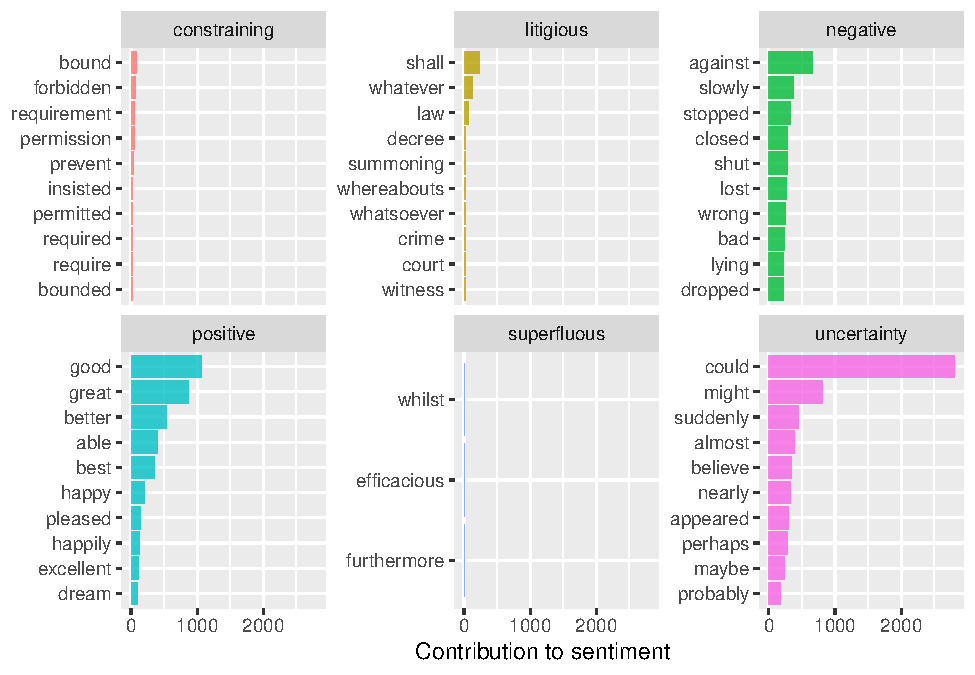
\includegraphics{Lab-7---Inference-for-Numerical-Data_files/figure-latex/unnamed-chunk-18-1.pdf}

The confidence interval for the difference between the weights of those
who exercise at least three times a week and those who don't can also be
calculated on the null distribution with a Welch Two Sample t-test. This
assumes the variances of the two are not equivalent.

\begin{Shaded}
\begin{Highlighting}[]
\KeywordTok{t.test}\NormalTok{(}\DataTypeTok{data =}\NormalTok{ yrbss, weight }\OperatorTok{~}\StringTok{ }\NormalTok{physical_3plus)}
\end{Highlighting}
\end{Shaded}

\begin{verbatim}
## 
##  Welch Two Sample t-test
## 
## data:  weight by physical_3plus
## t = -5.353, df = 7478.8, p-value = 8.908e-08
## alternative hypothesis: true difference in means is not equal to 0
## 95 percent confidence interval:
##  -2.424441 -1.124728
## sample estimates:
##  mean in group no mean in group yes 
##          66.67389          68.44847
\end{verbatim}

We can also calculate the intervals manually using the equation
\(\bar{x}\pm t_{df}*\frac{s}{\sqrt{n}}\) for comparison but to do so we
need some parameters first.

Find the standard deviation of each category.

\begin{Shaded}
\begin{Highlighting}[]
\NormalTok{yrbss }\OperatorTok\StringTok{ }
\StringTok{  }\KeywordTok{group_by}\NormalTok{(physical_3plus) }\OperatorTok\StringTok{ }
\StringTok{  }\KeywordTok{summarise}\NormalTok{(}\DataTypeTok{sd_weight =} \KeywordTok{sd}\NormalTok{(weight, }\DataTypeTok{na.rm =} \OtherTok{TRUE}\NormalTok{))}
\end{Highlighting}
\end{Shaded}

\begin{verbatim}
## `summarise()` ungrouping output (override with `.groups` argument)
\end{verbatim}

\begin{verbatim}
## # A tibble: 3 x 2
##   physical_3plus sd_weight
##   <chr>              <dbl>
## 1 no                  17.6
## 2 yes                 16.5
## 3 <NA>                17.6
\end{verbatim}

The standard deviation is 17.638 for those who do are not physically
active at least 3 days per week and 16.478 for those who are.

Find the mean of the weights in each category.

\begin{Shaded}
\begin{Highlighting}[]
\NormalTok{yrbss }\OperatorTok\StringTok{ }
\StringTok{  }\KeywordTok{group_by}\NormalTok{(physical_3plus) }\OperatorTok\StringTok{ }
\StringTok{  }\KeywordTok{summarise}\NormalTok{(}\DataTypeTok{mean_weight =} \KeywordTok{mean}\NormalTok{(weight, }\DataTypeTok{na.rm =} \OtherTok{TRUE}\NormalTok{))}
\end{Highlighting}
\end{Shaded}

\begin{verbatim}
## `summarise()` ungrouping output (override with `.groups` argument)
\end{verbatim}

\begin{verbatim}
## # A tibble: 3 x 2
##   physical_3plus mean_weight
##   <chr>                <dbl>
## 1 no                    66.7
## 2 yes                   68.4
## 3 <NA>                  69.9
\end{verbatim}

This agrees with the results from earlier that the mean weight is 66.674
for those who do are not physically active at least 3 days per week and
68.448 for those who are.

Lastly, the sample size of the whole was calculated as 13,583 with
missing values. We want the sample sizes of each category.

\begin{Shaded}
\begin{Highlighting}[]
\NormalTok{yrbss }\OperatorTok\StringTok{ }
\StringTok{  }\KeywordTok{group_by}\NormalTok{(physical_3plus) }\OperatorTok\StringTok{ }
\StringTok{  }\KeywordTok{summarise}\NormalTok{(}\DataTypeTok{freq =} \KeywordTok{table}\NormalTok{(weight)) }\OperatorTok
\StringTok{  }\KeywordTok{summarise}\NormalTok{(}\DataTypeTok{n =} \KeywordTok{sum}\NormalTok{(freq))}
\end{Highlighting}
\end{Shaded}

\begin{verbatim}
## `summarise()` regrouping output by 'physical_3plus' (override with `.groups` argument)
\end{verbatim}

\begin{verbatim}
## `summarise()` ungrouping output (override with `.groups` argument)
\end{verbatim}

\begin{verbatim}
## # A tibble: 3 x 2
##   physical_3plus     n
##   <chr>          <int>
## 1 no              4022
## 2 yes             8342
## 3 <NA>             215
\end{verbatim}

For example, the sample size of those who were physically active for at
least 3 days per week is 8,342 while the sample size of those who were
not physically active for at least 3 days per week is 4,022. Missing
values were not included since they do not convey any meaning here.

We can now calculate the confidence interval of each category using a
95\% confidence level.

\begin{Shaded}
\begin{Highlighting}[]
\NormalTok{x_not3plus <-}\StringTok{ }\FloatTok{66.67389}
\NormalTok{n_not3plus <-}\StringTok{ }\DecValTok{4022}
\NormalTok{s_not3plus <-}\StringTok{ }\FloatTok{17.63805}
\NormalTok{x_3plus <-}\StringTok{ }\FloatTok{68.44847}
\NormalTok{n_3plus <-}\StringTok{ }\DecValTok{8342}
\NormalTok{s_3plus <-}\StringTok{ }\FloatTok{16.47832}
\CommentTok{# At 95% confidence level where n is so large it is ~= z* of}
\CommentTok{# normal distribution}
\NormalTok{t =}\StringTok{ }\FloatTok{1.96}

\CommentTok{# Not physically active 3 plus days per week}
\NormalTok{upper_ci_not <-}\StringTok{ }\NormalTok{x_not3plus }\OperatorTok{+}\StringTok{ }\NormalTok{t}\OperatorTok{*}\NormalTok{(s_not3plus}\OperatorTok{/}\KeywordTok{sqrt}\NormalTok{(n_not3plus))}
\NormalTok{lower_ci_not <-}\StringTok{ }\NormalTok{x_not3plus }\OperatorTok{-}\StringTok{ }\NormalTok{t}\OperatorTok{*}\NormalTok{(s_not3plus}\OperatorTok{/}\KeywordTok{sqrt}\NormalTok{(n_not3plus))}

\CommentTok{# physically active 3 plus days per week}
\NormalTok{upper_ci <-}\StringTok{ }\NormalTok{x_3plus }\OperatorTok{+}\StringTok{ }\NormalTok{t}\OperatorTok{*}\NormalTok{(s_3plus}\OperatorTok{/}\KeywordTok{sqrt}\NormalTok{(n_3plus))}
\NormalTok{lower_ci <-}\StringTok{ }\NormalTok{x_3plus }\OperatorTok{-}\StringTok{ }\NormalTok{t}\OperatorTok{*}\NormalTok{(s_3plus}\OperatorTok{/}\KeywordTok{sqrt}\NormalTok{(n_3plus))}

\NormalTok{upper_ci_not}
\end{Highlighting}
\end{Shaded}

\begin{verbatim}
## [1] 67.219
\end{verbatim}

\begin{Shaded}
\begin{Highlighting}[]
\NormalTok{lower_ci_not}
\end{Highlighting}
\end{Shaded}

\begin{verbatim}
## [1] 66.12878
\end{verbatim}

\begin{Shaded}
\begin{Highlighting}[]
\NormalTok{upper_ci}
\end{Highlighting}
\end{Shaded}

\begin{verbatim}
## [1] 68.80209
\end{verbatim}

\begin{Shaded}
\begin{Highlighting}[]
\NormalTok{lower_ci}
\end{Highlighting}
\end{Shaded}

\begin{verbatim}
## [1] 68.09485
\end{verbatim}

We can be 95\% confident that those students who exercise at least three
times a week have an average weight between 68.095 kg and 68.802 kg. We
can also be confident that those students who do not exercise at least
three times a week have an average weight between 66.129 kg and 67.219
kg.

\hypertarget{exercise-8}{%
\subsubsection{Exercise 8}\label{exercise-8}}

Calculate a 95\% confidence interval for the average height in meters
(height) and interpret it in context.

\begin{Shaded}
\begin{Highlighting}[]
\CommentTok{# Verifying sum of frequency / counts = n without NAs}
\NormalTok{table_height <-}\StringTok{ }\KeywordTok{as.data.frame}\NormalTok{(}\KeywordTok{table}\NormalTok{(yrbss}\OperatorTok{$}\NormalTok{height))}
\NormalTok{freq_height <-}\StringTok{ }\KeywordTok{sum}\NormalTok{(table_height}\OperatorTok{$}\NormalTok{Freq)}

\NormalTok{x_height <-}\StringTok{ }\KeywordTok{mean}\NormalTok{(yrbss}\OperatorTok{$}\NormalTok{height, }\DataTypeTok{na.rm =} \OtherTok{TRUE}\NormalTok{)}
\NormalTok{sd_height <-}\StringTok{ }\KeywordTok{sd}\NormalTok{(yrbss}\OperatorTok{$}\NormalTok{height, }\DataTypeTok{na.rm =} \OtherTok{TRUE}\NormalTok{)}
\NormalTok{n_height <-}\StringTok{ }\NormalTok{yrbss }\OperatorTok\StringTok{ }
\StringTok{  }\KeywordTok{summarise}\NormalTok{(}\DataTypeTok{freq =} \KeywordTok{table}\NormalTok{(height)) }\OperatorTok
\StringTok{  }\KeywordTok{summarise}\NormalTok{(}\DataTypeTok{n =} \KeywordTok{sum}\NormalTok{(freq, }\DataTypeTok{na.rm =} \OtherTok{TRUE}\NormalTok{))}

\NormalTok{upper_ci_height <-}\StringTok{ }\NormalTok{x_height }\OperatorTok{+}\StringTok{ }\NormalTok{t}\OperatorTok{*}\NormalTok{(sd_height}\OperatorTok{/}\KeywordTok{sqrt}\NormalTok{(n_height))}
\NormalTok{lower_ci_height <-}\StringTok{ }\NormalTok{x_height }\OperatorTok{-}\StringTok{ }\NormalTok{t}\OperatorTok{*}\NormalTok{(sd_height}\OperatorTok{/}\KeywordTok{sqrt}\NormalTok{(n_height))}
\NormalTok{upper_ci_height}
\end{Highlighting}
\end{Shaded}

\begin{verbatim}
##          n
## 1 1.693071
\end{verbatim}

\begin{Shaded}
\begin{Highlighting}[]
\NormalTok{lower_ci_height}
\end{Highlighting}
\end{Shaded}

\begin{verbatim}
##          n
## 1 1.689411
\end{verbatim}

We can be 95\% confident that the average height of the students in this
population is between 1.689m and 1.693m.

\hypertarget{exercise-9}{%
\subsubsection{Exercise 9}\label{exercise-9}}

Calculate a new confidence interval for the same parameter at the 90\%
confidence level. Comment on the width of this interval versus the one
obtained in the previous exercise.

\begin{Shaded}
\begin{Highlighting}[]
\CommentTok{# At 90% confidence level where n is so large it is ~= z-score of normal distribution }
\NormalTok{t_}\DecValTok{90}\NormalTok{ <-}\StringTok{ }\FloatTok{1.645}
\NormalTok{upper_ci_height_}\DecValTok{90}\NormalTok{ <-}\StringTok{ }\NormalTok{x_height }\OperatorTok{+}\StringTok{ }\NormalTok{t_}\DecValTok{90}\OperatorTok{*}\NormalTok{(sd_height}\OperatorTok{/}\KeywordTok{sqrt}\NormalTok{(n_height))}
\NormalTok{lower_ci_height_}\DecValTok{90}\NormalTok{ <-}\StringTok{ }\NormalTok{x_height }\OperatorTok{-}\StringTok{ }\NormalTok{t_}\DecValTok{90}\OperatorTok{*}\NormalTok{(sd_height}\OperatorTok{/}\KeywordTok{sqrt}\NormalTok{(n_height))}
\NormalTok{upper_ci_height_}\DecValTok{90}
\end{Highlighting}
\end{Shaded}

\begin{verbatim}
##          n
## 1 1.692777
\end{verbatim}

\begin{Shaded}
\begin{Highlighting}[]
\NormalTok{lower_ci_height_}\DecValTok{90}
\end{Highlighting}
\end{Shaded}

\begin{verbatim}
##          n
## 1 1.689705
\end{verbatim}

The new confidence interval is 1.689705 to 1.692777. Our intervals at a
95\% confidence level were 1.689411 and 1.693071. We can find the
difference in these two confidence intervals and compare 90\% to 95\%
confidence.

\begin{Shaded}
\begin{Highlighting}[]
\NormalTok{rng_hgt_}\DecValTok{95}\NormalTok{ <-}\StringTok{ }\NormalTok{(upper_ci_height }\OperatorTok{-}\StringTok{ }\NormalTok{lower_ci_height)}
\NormalTok{rng_hgt_}\DecValTok{90}\NormalTok{ <-}\StringTok{ }\NormalTok{(upper_ci_height_}\DecValTok{90} \OperatorTok{-}\StringTok{ }\NormalTok{lower_ci_height_}\DecValTok{90}\NormalTok{)}
\NormalTok{rng_hgt_}\DecValTok{95}
\end{Highlighting}
\end{Shaded}

\begin{verbatim}
##             n
## 1 0.003659302
\end{verbatim}

\begin{Shaded}
\begin{Highlighting}[]
\NormalTok{rng_hgt_}\DecValTok{90}
\end{Highlighting}
\end{Shaded}

\begin{verbatim}
##           n
## 1 0.0030712
\end{verbatim}

As expected, the 95\% confidence interval has a slightly larger range
than the confidence interval 90\%. This larger range is necessary to be
more certain about the population parameter.

\hypertarget{exercise-10}{%
\subsubsection{Exercise 10}\label{exercise-10}}

Conduct a hypothesis test evaluating whether the average height is
different for those who exercise at least three times a week and those
who don't.

Null hypothesis: There is no difference in the average height of those
who are physically active at least 3 days per week and those who are
not.

Alternative hypothesis: There is a difference in the average height of
those who are physically active at least 3 days per week and those who
are not.

\begin{Shaded}
\begin{Highlighting}[]
\NormalTok{obs_diff_hgt <-}\StringTok{ }\NormalTok{yrbss }\OperatorTok
\StringTok{  }\KeywordTok{specify}\NormalTok{(height }\OperatorTok{~}\StringTok{ }\NormalTok{physical_3plus) }\OperatorTok
\StringTok{  }\KeywordTok{calculate}\NormalTok{(}\DataTypeTok{stat =} \StringTok{"diff in means"}\NormalTok{, }\DataTypeTok{order =} \KeywordTok{c}\NormalTok{(}\StringTok{"yes"}\NormalTok{, }\StringTok{"no"}\NormalTok{))}
\end{Highlighting}
\end{Shaded}

\begin{verbatim}
## Warning: Removed 1219 rows containing missing values.
\end{verbatim}

\begin{Shaded}
\begin{Highlighting}[]
\KeywordTok{set.seed}\NormalTok{(}\DecValTok{10152020}\NormalTok{)}
\NormalTok{null_dist_hgt <-}\StringTok{ }\NormalTok{yrbss }\OperatorTok
\StringTok{  }\KeywordTok{specify}\NormalTok{(height }\OperatorTok{~}\StringTok{ }\NormalTok{physical_3plus) }\OperatorTok
\StringTok{  }\KeywordTok{hypothesize}\NormalTok{(}\DataTypeTok{null =} \StringTok{"independence"}\NormalTok{) }\OperatorTok
\StringTok{  }\KeywordTok{generate}\NormalTok{(}\DataTypeTok{reps =} \DecValTok{1000}\NormalTok{, }\DataTypeTok{type =} \StringTok{"permute"}\NormalTok{) }\OperatorTok
\StringTok{  }\KeywordTok{calculate}\NormalTok{(}\DataTypeTok{stat =} \StringTok{"diff in means"}\NormalTok{, }\DataTypeTok{order =} \KeywordTok{c}\NormalTok{(}\StringTok{"yes"}\NormalTok{, }\StringTok{"no"}\NormalTok{))}
\end{Highlighting}
\end{Shaded}

\begin{verbatim}
## Warning: Removed 1219 rows containing missing values.
\end{verbatim}

\begin{Shaded}
\begin{Highlighting}[]
\KeywordTok{visualize}\NormalTok{(null_dist_hgt) }\OperatorTok{+}\StringTok{ }
\StringTok{  }\KeywordTok{shade_p_value}\NormalTok{(}\DataTypeTok{obs_stat =}\NormalTok{ obs_diff_hgt, }\DataTypeTok{direction =} \StringTok{"two_sided"}\NormalTok{)}
\end{Highlighting}
\end{Shaded}

\includegraphics{Lab-7---Inference-for-Numerical-Data_files/figure-latex/unnamed-chunk-27-1.pdf}

\begin{Shaded}
\begin{Highlighting}[]
\NormalTok{null_dist_hgt }\OperatorTok
\StringTok{  }\KeywordTok{get_p_value}\NormalTok{(}\DataTypeTok{obs_stat =}\NormalTok{ obs_diff_hgt, }\DataTypeTok{direction =} \StringTok{"two_sided"}\NormalTok{)}
\end{Highlighting}
\end{Shaded}

\begin{verbatim}
## Warning: Please be cautious in reporting a p-value of 0. This result is an
## approximation based on the number of `reps` chosen in the `generate()` step. See
## `?get_p_value()` for more information.
\end{verbatim}

\begin{verbatim}
## # A tibble: 1 x 1
##   p_value
##     <dbl>
## 1       0
\end{verbatim}

The p-value is very small, smaller than 0.05. At this level, we should
reject the null hypothesis.

\begin{Shaded}
\begin{Highlighting}[]
\KeywordTok{inference}\NormalTok{(}\DataTypeTok{data =}\NormalTok{ yrbss, }\DataTypeTok{y =}\NormalTok{ height, }\DataTypeTok{x =}\NormalTok{ physical_3plus,}
          \DataTypeTok{statistic =} \StringTok{"mean"}\NormalTok{,}
          \DataTypeTok{type =} \StringTok{"ci"}\NormalTok{, }
          \DataTypeTok{null =} \OtherTok{NULL}\NormalTok{, }
          \DataTypeTok{alternative =} \StringTok{"twosided"}\NormalTok{, }
          \DataTypeTok{method =} \StringTok{"theoretical"}\NormalTok{)}
\end{Highlighting}
\end{Shaded}

\begin{verbatim}
## Response variable: numerical, Explanatory variable: categorical (2 levels)
## n_no = 4022, y_bar_no = 1.6656, s_no = 0.1029
## n_yes = 8342, y_bar_yes = 1.7032, s_yes = 0.1033
## 95% CI (no - yes): (-0.0415 , -0.0337)
\end{verbatim}

\includegraphics{Lab-7---Inference-for-Numerical-Data_files/figure-latex/unnamed-chunk-28-1.pdf}

\begin{Shaded}
\begin{Highlighting}[]
\NormalTok{x_nhgt <-}\StringTok{ }\FloatTok{1.6665}
\NormalTok{n_nhgt <-}\StringTok{ }\DecValTok{4022}
\NormalTok{s_nhgt <-}\StringTok{ }\FloatTok{0.1029}
\NormalTok{x_yhgt <-}\StringTok{ }\FloatTok{1.7032}
\NormalTok{n_yhgt <-}\StringTok{ }\DecValTok{8342}
\NormalTok{s_yhgt <-}\StringTok{ }\FloatTok{0.1033}
\CommentTok{# At 95% confidence level where n is so large it is ~= z* of}
\CommentTok{# normal distribution}
\NormalTok{t =}\StringTok{ }\FloatTok{1.96}

\CommentTok{# Not physically active 3 plus days per week}
\NormalTok{upper_ci_nhgt <-}\StringTok{ }\NormalTok{x_nhgt }\OperatorTok{+}\StringTok{ }\NormalTok{t}\OperatorTok{*}\NormalTok{(s_nhgt}\OperatorTok{/}\KeywordTok{sqrt}\NormalTok{(n_nhgt))}
\NormalTok{lower_ci_nhgt <-}\StringTok{ }\NormalTok{x_nhgt }\OperatorTok{-}\StringTok{ }\NormalTok{t}\OperatorTok{*}\NormalTok{(s_nhgt}\OperatorTok{/}\KeywordTok{sqrt}\NormalTok{(n_nhgt))}

\CommentTok{# physically active 3 plus days per week}
\NormalTok{upper_ci_yhgt <-}\StringTok{ }\NormalTok{x_yhgt }\OperatorTok{+}\StringTok{ }\NormalTok{t}\OperatorTok{*}\NormalTok{(s_yhgt}\OperatorTok{/}\KeywordTok{sqrt}\NormalTok{(n_yhgt))}
\NormalTok{lower_ci_yhgt <-}\StringTok{ }\NormalTok{x_yhgt }\OperatorTok{-}\StringTok{ }\NormalTok{t}\OperatorTok{*}\NormalTok{(s_yhgt}\OperatorTok{/}\KeywordTok{sqrt}\NormalTok{(n_yhgt))}

\NormalTok{upper_ci_nhgt}
\end{Highlighting}
\end{Shaded}

\begin{verbatim}
## [1] 1.66968
\end{verbatim}

\begin{Shaded}
\begin{Highlighting}[]
\NormalTok{lower_ci_nhgt}
\end{Highlighting}
\end{Shaded}

\begin{verbatim}
## [1] 1.66332
\end{verbatim}

\begin{Shaded}
\begin{Highlighting}[]
\NormalTok{upper_ci_yhgt}
\end{Highlighting}
\end{Shaded}

\begin{verbatim}
## [1] 1.705417
\end{verbatim}

\begin{Shaded}
\begin{Highlighting}[]
\NormalTok{lower_ci_yhgt }
\end{Highlighting}
\end{Shaded}

\begin{verbatim}
## [1] 1.700983
\end{verbatim}

We can be 95\% confident that the average height of students who are
physically active at least 3 days per week is between 1.705 and 1.701
while the average height of students who are not physically active at
least 3 days per week is between 1.670 and 1.663.

\hypertarget{exercise-11}{%
\subsubsection{Exercise 11}\label{exercise-11}}

Now, a non-inference task: Determine the number of different options
there are in the dataset for the hours\_tv\_per\_school\_day there are.

If the question is referring to the number of combinations (or options)
of the variable hours\_tv\_per\_school\_day, then the answer would
depend on whether or not the order of the options matter and if we
should repeat or replace the variables once they are used. We can easily
calculate the number of different variables including
hours\_tv\_per\_school\_day at 14 and see each of their labels below.

\begin{Shaded}
\begin{Highlighting}[]
\KeywordTok{ncol}\NormalTok{(yrbss)}
\end{Highlighting}
\end{Shaded}

\begin{verbatim}
## [1] 14
\end{verbatim}

\begin{Shaded}
\begin{Highlighting}[]
\KeywordTok{colnames}\NormalTok{(yrbss)}
\end{Highlighting}
\end{Shaded}

\begin{verbatim}
##  [1] "age"                      "gender"                  
##  [3] "grade"                    "hispanic"                
##  [5] "race"                     "height"                  
##  [7] "weight"                   "helmet_12m"              
##  [9] "text_while_driving_30d"   "physically_active_7d"    
## [11] "hours_tv_per_school_day"  "strength_training_7d"    
## [13] "school_night_hours_sleep" "physical_3plus"
\end{verbatim}

There are also only 14 different options if the variable
hours\_tv\_per\_school\_day can only be paired with exactly one other
variable from the dataset only once and including itself.

If the question is referring to the number of options within the
variable hours\_tv\_per\_school\_day then we can calculate the quantity
of unique values for this particular variable in the dataset.

\begin{Shaded}
\begin{Highlighting}[]
\KeywordTok{unique}\NormalTok{(yrbss}\OperatorTok{$}\NormalTok{hours_tv_per_school_day)}
\end{Highlighting}
\end{Shaded}

\begin{verbatim}
## [1] "5+"           "2"            "3"            "do not watch" "<1"          
## [6] "4"            "1"            NA
\end{verbatim}

\begin{Shaded}
\begin{Highlighting}[]
\KeywordTok{length}\NormalTok{(}\KeywordTok{unique}\NormalTok{(yrbss}\OperatorTok{$}\NormalTok{hours_tv_per_school_day))}
\end{Highlighting}
\end{Shaded}

\begin{verbatim}
## [1] 8
\end{verbatim}

We can see the options here are ``do not watch'', ``\textless1'', 1, 2,
3, 4, 5+, and NA. If we are to include missing values as an option
within this dataset then we are left with 8 options of the variable
hours\_tv\_per\_school\_day. If we were to remove the missing values as
an option in the variable then the answer is 7 options without NA.

\hypertarget{exercise-12}{%
\subsubsection{Exercise 12}\label{exercise-12}}

Come up with a research question evaluating the relationship between
height or weight and sleep. Formulate the question in a way that it can
be answered using a hypothesis test and/or a confidence interval. Report
the statistical results, and also provide an explanation in plain
language. Be sure to check all assumptions, state your α level, and
conclude in context.

Setup:

Null hypothesis: The average weight of students has no affect on the
average number of hours of sleep students receive on school nights.

Alternative hypothesis: The average weight of students has an affect on
the average number of hours of sleep students receive on school nights.

An analysis of variance(ANOVA) would work best for this to determine if
the means of all the groups are different from the null. We know the
data are independent already and are approximately normal. Since we have
more than two means to compare, this is a good place to start. To be
more specific, there are 8 groups to find means of.

\begin{Shaded}
\begin{Highlighting}[]
\KeywordTok{unique}\NormalTok{(yrbss}\OperatorTok{$}\NormalTok{school_night_hours_sleep)}
\end{Highlighting}
\end{Shaded}

\begin{verbatim}
## [1] "8"   "6"   "<5"  "9"   "10+" "7"   "5"   NA
\end{verbatim}

\begin{Shaded}
\begin{Highlighting}[]
\KeywordTok{length}\NormalTok{(}\KeywordTok{unique}\NormalTok{(yrbss}\OperatorTok{$}\NormalTok{school_night_hours_sleep))}
\end{Highlighting}
\end{Shaded}

\begin{verbatim}
## [1] 8
\end{verbatim}

We can call these eight options in the school\_night\_hours\_sleep
variable the sleeping groups. For each sleeping group we will find the
mean and other statistics. First, let's look at a boxplot for outliers.

\begin{Shaded}
\begin{Highlighting}[]
\KeywordTok{ggplot}\NormalTok{(yrbss, }\KeywordTok{aes}\NormalTok{(}\DataTypeTok{x =}\NormalTok{ weight, }\DataTypeTok{y =}\NormalTok{ school_night_hours_sleep)) }\OperatorTok{+}\StringTok{ }\KeywordTok{geom_boxplot}\NormalTok{()}
\end{Highlighting}
\end{Shaded}

\begin{verbatim}
## Warning: Removed 1004 rows containing non-finite values (stat_boxplot).
\end{verbatim}

\includegraphics{Lab-7---Inference-for-Numerical-Data_files/figure-latex/unnamed-chunk-33-1.pdf}

Based on the boxplot, all of the medians appear similar with some subtle
variations. Each sleeping group also has similar IQRs but we should take
a closer look.

\begin{Shaded}
\begin{Highlighting}[]
\NormalTok{desc <-}\StringTok{ }\KeywordTok{describeBy}\NormalTok{(yrbss}\OperatorTok{$}\NormalTok{weight, yrbss}\OperatorTok{$}\NormalTok{school_night_hours_sleep, }\DataTypeTok{mat=}\OtherTok{TRUE}\NormalTok{)[,}\KeywordTok{c}\NormalTok{(}\DecValTok{2}\NormalTok{,}\DecValTok{4}\NormalTok{,}\DecValTok{5}\NormalTok{,}\DecValTok{6}\NormalTok{)]}
\NormalTok{desc}\OperatorTok{$}\NormalTok{Var <-}\StringTok{ }\NormalTok{desc}\OperatorTok{$}\NormalTok{sd}\OperatorTok{^}\DecValTok{2}
\KeywordTok{print}\NormalTok{(desc, }\DataTypeTok{row.names=}\OtherTok{FALSE}\NormalTok{)}
\end{Highlighting}
\end{Shaded}

\begin{verbatim}
##  group1    n     mean       sd      Var
##      <5  859 70.29700 19.47970 379.4586
##     10+  255 69.29251 19.92961 397.1895
##       5 1378 68.41806 17.47753 305.4639
##       6 2496 68.33318 17.12553 293.2838
##       7 3283 67.43457 16.12185 259.9140
##       8 2505 67.45745 16.52393 273.0401
##       9  705 65.55898 15.87743 252.0929
\end{verbatim}

The sample sizes of each sleeping group are greater than 30 and based on
the boxplots and means calculated for each sleeping group, there are
very few particularly extreme values. There is clear variation in
sleeping groups, however, they are close enough to perform an anova.

\begin{Shaded}
\begin{Highlighting}[]
\NormalTok{aov.out <-}\StringTok{ }\KeywordTok{aov}\NormalTok{(}\DataTypeTok{data=}\NormalTok{yrbss, weight }\OperatorTok{~}\StringTok{ }\NormalTok{school_night_hours_sleep )}
\KeywordTok{summary}\NormalTok{(aov.out)}
\end{Highlighting}
\end{Shaded}

\begin{verbatim}
##                             Df  Sum Sq Mean Sq F value  Pr(>F)    
## school_night_hours_sleep     6   11333    1889   6.581 5.9e-07 ***
## Residuals                11474 3293032     287                    
## ---
## Signif. codes:  0 '***' 0.001 '**' 0.01 '*' 0.05 '.' 0.1 ' ' 1
## 2102 observations deleted due to missingness
\end{verbatim}

This produces a p-value that is significant to the 0.001 level. This
provides strong evidence that we should reject the null hypothesis in
favor of the alternative. In other words, the average weight of students
appears to have an affect on the average number of hours of sleep
students receive on school nights. \ldots{}

\end{document}
